\documentclass[crop,border={2pt 2pt 2pt 2pt},tikz]{standalone}
\usepackage{braket}
\usepackage{bbold}
\usepackage{bm}
\usepackage{amsmath}
\usepackage{tikz-3dplot}
\usepackage{physics}

\usetikzlibrary{backgrounds,decorations.markings, calc}
\tikzset{>=latex}
\tikzset{->-/.style={decoration={
  markings,
  mark=at position .55 with {\arrow{>}}},postaction={decorate}}}
\begin{document}
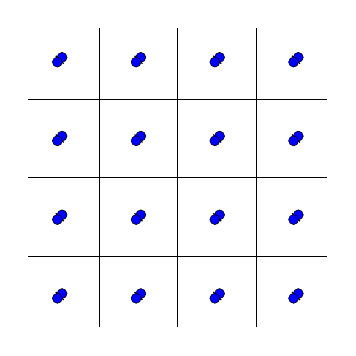
\begin{tikzpicture}[line join = round]
    \draw[black] (0.1,0.1) grid(3.9,3.9);

    \foreach \i in {0,...,3} 
    \foreach \j in {0,...,3} 
    {
    \draw[black] (\i+0.45,\j+0.45) -- (\i+0.55,\j+0.55);
    \draw[black] (\i+0.45,\j+0.55) -- (\i+0.55,\j+0.45);
    }
    \foreach \i in {0,...,3} 
    \foreach \j in {0,...,3} 
    {
    \draw[fill=blue, very thin] (\i+0.53 ,\j+0.53) circle (1.8pt);
    \draw[fill=blue, very thin] (\i+0.47 ,\j+0.47) circle (1.8pt);
    }
\end{tikzpicture}
\end{document}